\documentclass[a4paper,twocolumn,10pt]{article}
\usepackage[utf8]{inputenc}
\usepackage{graphicx}
\usepackage{amsmath}



%opening
\title{Occupancy Detection:\ The Ins And Outs}

\author{
    Arote, Uddhav\\
    \texttt{uddhava@cse.iitb.ac.in}\and
    Palani, Kartik\\
    \texttt{kartik@cse.iitb.ac.in}\and
    Nasir, Nabeel\\
    \texttt{nabeeln@cse.iitb.ac.in}\and
    Chil Prakash, Vivek\\
    \texttt{vivekcprakash@cse.iitb.ac.in}
}

\begin{document}

\maketitle

\begin{abstract}


  % This is the comment, which won't come up on the pdf
  % This is single line comment


  Virtualization\cite{Boney96} is the hot topic in the operating systems 
  these days. It is useful in many scenarios: server consolidation,
  virtual test environments, and for Linux enthusiasts who
  still cannot decide upon the which distribution is best.
  
  \noindent The Kernel Virtual Machine, or \textbf{kvm} is a new Linux
  subsystem which leverages these virtualization extensions
  to add a virtual machine monitor (or hypervisor) capability to Linux.
\end{abstract}

\section{Background}
  Virtualization is the hot topic in the operating systems\cite{MG} 
  these days. It is useful in many scenarios: server consolidation,
  virtual test environments, and for Linux enthusiasts who
  still cannot decide upon the which distribution is best.
  
  \noindent The Kernel Virtual Machine, or \textbf{kvm} is a new Linux
  subsystem which leverages these virtualization extensions
  to add a virtual machine monitor (or hypervisor) capability to Linux.

  
  \noindent Virtualization is the hot topic in the operating systems 
  these days. It is useful in many scenarios: server consolidation,
  virtual test environments, and for Linux enthusiasts who
  still cannot decide upon the which distribution is best.
  
  \noindent The Kernel Virtual Machine, or \textbf{kvm} is a new Linux
  subsystem which leverages these virtualization extensions
  to add a virtual machine monitor (or hypervisor) capability to Linux.

  
\section{x86 virtualization}
Virtualization is the hot topic in the operating systems 
  these days. It is useful in many scenarios: server consolidation,
  virtual test environments, and for Linux enthusiasts who
  still cannot decide upon the which distribution is best.
  
  \noindent The Kernel Virtual Machine, or \textbf{kvm} is a new Linux
  subsystem which leverages these virtualization extensions
  to add a virtual machine monitor (or hypervisor) capability to Linux.

  
   \begin{figure}[h]
     \centering
      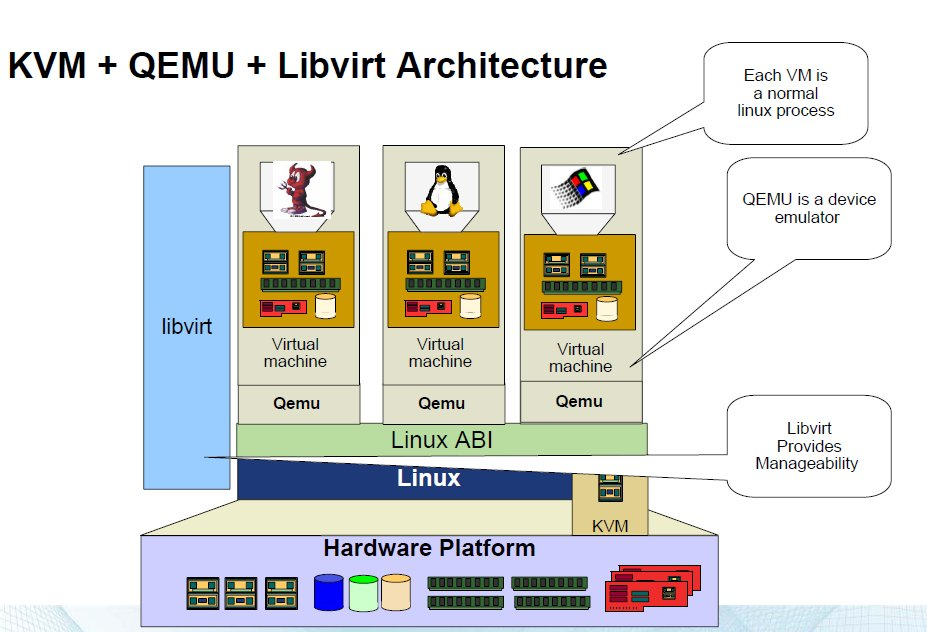
\includegraphics[width=90mm]{arch.jpg}
      \caption{kvm: architecture}
      \label{arch}
   \end{figure}

  
  \noindent Virtualization is the hot topic in the operating systems 
  these days. It is useful in many scenarios: server consolidation,
  virtual test environments, and for Linux enthusiasts who
  still cannot decide upon the which distribution is best.
  
  \noindent The Kernel Virtual Machine, or \textbf{kvm} is a new Linux
  subsystem which leverages these virtualization extensions
  to add a virtual machine monitor (or hypervisor) capability to Linux.
  \pagebreak
  
  \begin{center}
\begin{table*}[ht]
{\small
\hfill{}
\begin{tabular}{|l|l|c|c|c|c|c|c|c|}
\hline
\textbf{Hello}&\textbf{Hello}& \multicolumn{7}{|c|}{\textbf{Hello}}\\
\cline{3-9}
\hline
AAAAA&AAAAA&AAAAA&AAAAA&AAAAA&AAAAA&AAAAA&AAAAA&AAAAA\\
BBBBB&BBBBB&BBBBB&BBBBB&BBBBB&BBBBB&BBBBB&BBBBB&BBBBB\\
AAAAA&AAAAA&AAAAA&AAAAA&AAAAA&AAAAA&AAAAA&AAAAA&AAAAA\\
BBBBB&BBBBB&BBBBB&BBBBB&BBBBB&BBBBB&BBBBB&BBBBB&BBBBB\\
\hline
\end{tabular}}
\hfill{}
\caption{Table Name}
\label{tb:tablename}
\end{table*}
\end{center}
\section{MMU virtualization}
Virtualization is the hot topic in the operating systems 
  these days. It is useful in many scenarios: server consolidation\footnote{Consolidate all servers on one machine},
  virtual test environments, and for Linux enthusiasts who
  still cannot decide upon the which distribution is best.
  
  \begin{figure}
   \centering
   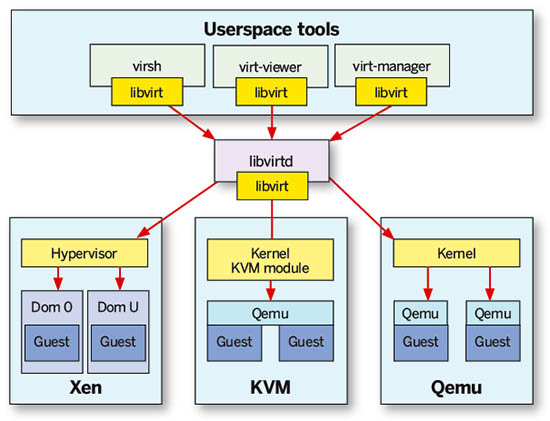
\includegraphics[width=60mm]{arch1.jpg}
   \caption{YAkvmA}
   \label{arch1}
  \end{figure}

  
  \noindent The Kernel Virtual Machine, or \textbf{kvm} is a new Linux
  subsystem which leverages these virtualization extensions
  to add a virtual machine monitor (or hypervisor) capability to Linux.
 
  \noindent Virtualization is the  hot topic in the operating systems 
  these days. It is useful in many scenarios: server consolidation,
  virtual test environments, and for Linux enthusiasts who
  still cannot decide upon the which distribution is best.
  
 \begin{displaymath}\int\frac{d\theta + \pi/2 + \sum \limits_{i=2}^{10} i^2 + i\theta ^2 + i/\pi }{1+\theta^2}=\tan^{-1} \theta + C \hspace{10pt}(2)
  \end{displaymath}

 

  
  \noindent The Kernel Virtual Machine\footnote{kvm, is a Linux subsystem}, or \textbf{kvm} is a new Linux
  subsystem which leverages these virtualization extensions
  to add a virtual machine monitor (or hypervisor) capability to Linux. The architecture is show in fig.\ref{arch1}

   \subsection{Shadow Paging}
    \noindent Virtualization is \newline the hot topic in the operating systems 
  these days. It is useful in many scenarios: server consolidation,
  virtual test environments, and for Linux enthusiasts who
  still cannot decide upon the which distribution is best.
  
  \noindent The Kernel Virtual Machine, or \textbf{kvm} is a new Linux
  subsystem which leverages these virtualization extensions
  to add a virtual machine monitor (or hypervisor) capability to Linux.
   
   \subsection{Direct Mapping}
   
    \noindent Virtualization is the hot topic in the operating systems 
  these days. It is useful in many scenarios: server consolidation,
  virtual test environments, and for Linux enthusiasts who
  still cannot decide upon the which distribution\cite{troy1} is best.
    
  \noindent The Kernel Virtual Machine, or \textbf{kvm} is a new Linux
  subsystem which leverages these virtualization extensions
  to add a virtual machine monitor (or hypervisor) capability to Linux.
   
   \subsection{Hardware assisted Paging}
    \noindent Virtualization is the hot topic in the operating systems 
  these days. It is useful in many scenarios: server consolidation,
  virtual test environments, and for Linux enthusiasts who
  still cannot decide upon the which distribution is best.
  
   \begin{displaymath}\frac{n!}{k!(n-k)!}=
  \binom{n}{k}
  \end{displaymath}
  
  \noindent The Kernel Virtual Machine, or \textbf{kvm} is a new Linux
  subsystem which leverages these virtualization extensions
  to add a virtual machine monitor\cite{troy} (or hypervisor) capability to Linux.
  
 \section{Types of Virtualization}
 \begin{enumerate}
  \item Full Virtualization
  \begin{itemize}
   \item x86
   \item MMU
   \item NIC
   \item IO
  \end{itemize}
  \item Para Virtualization
  \item Hardware Assisted Virtualization
 \end{enumerate}
 
 %\documentclass[first.tex]{subfile}
%\begin{document}
 \section{x86 Hardware Virtualization Techniques}
  x86 hardware is difficult to virtualize because few instructions\cite{ER}
  do not trap when executed in different privilege level. Follow the table \ref{table:virtualization 1} on page \pageref{table:virtualization 1}
  \noindent Virtualization is the hot topic in the operating systems 
  these days. It is useful in many scenarios: server consolidation,
  virtual test environments, and for Linux enthusiasts who
  still \begin{math}
          a + b * \pi + \theta + \sum\limits_{i=2}^{10}\frac{n!}{k!} + \forall + \leq + \geq =10
        \end{math}
 cannot decide upon the which distribution is best.
  
  
  
  \noindent The Kernel Virtual Machine, or \textbf{kvm} is a new Linux
  subsystem which leverages these virtualization extensions
  to add a virtual machine monitor (or hypervisor) capability to Linux.
  
  \noindent Virtualization is the hot topic in the operating systems 
  these days. It is useful in many scenarios: server consolidation,
  virtual test environments, and for Linux enthusiasts who
  still cannot decide upon the which distribution is best.
  
  \noindent The Kernel Virtual Machine, or \textbf{kvm} is a new Linux
  subsystem which leverages these virtualization extensions
  to add a virtual machine monitor (or hypervisor) capability to Linux.
  
 \begin{table}[ht]
  \centering
  \begin{tabular}{l r r r}
  \hline
  Hardware & I & II & III\\[0.5ex]
  \hline
  a & 1 & 2 & 3\\
  b & 1 & 2 & 3\\
  c & 1 & 2 & 3\\
  d & 1 & 2 & 3\\
  \hline
  \end{tabular}
  \caption{Virtualization I}
  \label{table:virtualization 1}
 \end{table}

  \noindent The Kernel Virtual Machine\cite{SH:13}, or \textbf{kvm} is a new Linux
  subsystem which leverages these virtualization extensions
  to add a virtual machine monitor (or hypervisor) capability to Linux.
  
  \noindent Virtualization is the hot topic in the operating systems 
  these days \cite{google} \cite{linux} \cite{xen}. It is useful in many scenarios: server consolidation,
  virtual test environments, and for Linux\footnote{Linux is best operating system ever} enthusiasts who
  still cannot decide upon the which distribution is best.
  \begin{table}[ht]
  \centering
  \begin{tabular}{l r r r r r}
  \hline
  Software & I & II & III & IV & V\\[0.4ex]
  \hline
  a & 1 & 2 & 3 & test & hello\\
  b & 1 & 2 & 3 & test & hello\\
  c & 1 & 2 & 3 & test & hello\\
  d & 1 & 2 & 3 & test & hello\\
  \hline
  \end{tabular}
  \caption{Virtualization II}

 \end{table}
%\end{document}


  
  
%%%%%%%%%%% Example 1%%%%%%%%%%%%%%%%%%%%%%%%%%%
\begin{thebibliography}{100} % 100 is a random guess of the total number of
%references

\bibitem{Boney96} Boney, L., Tewfik, A.H., and Hamdy, K.N., ``Digital
Watermarks for Audio Signals,"\emph{Proceedings of the Third IEEE
International Conference on Multimedia}, pp. 473-480, June 1996.

\bibitem{MG} Boney, L., Tewfik, A.H., and Hamdy, K.N., ``Digital
Watermarks for Audio Signals,"\emph{Proceedings of the Third IEEE
International Conference on Multimedia}, pp. 473-480, June 1996.

\bibitem{HK} Boney, L., Tewfik, A.H., and Hamdy, K.N., ``Digital
Watermarks for Audio Signals,"\emph{Proceedings of the Third IEEE
International Conference on Multimedia}, pp. 473-480, June 1996.

\bibitem{troy}  D A Troy and S H Zweben, {\em Measuring the Quality of
Structured Designs}, Journal of Systems and Software, {\bf 2}, 1981, 113--120

\bibitem{Zweben}  D A Troy and S H Zweben, {\em Measuring the Quality of
Structured Designs}, Journal of Systems and Software, {\bf 2}, 1981, 113--120

\bibitem{troy1}  D A Troy and S H Zweben, {\em Measuring the Quality of
Structured Designs}, Journal of Systems and Software, {\bf 2}, 1981, 113--120

\bibitem{google} http://www.google.com
\bibitem{linux} http://www.linux.com
\bibitem{xen} http://www.xenproject.org
\end{thebibliography}
  
  
  
\end{document}
